% https://tex.stackexchange.com/questions/192424/pgfplots-single-legend-in-a-group-plot

\documentclass[margin=5mm]{standalone}
\usepackage{pgfplots}
\usetikzlibrary{matrix}
\usepgfplotslibrary{groupplots}
\pgfplotsset{compat=newest}
\begin{document}

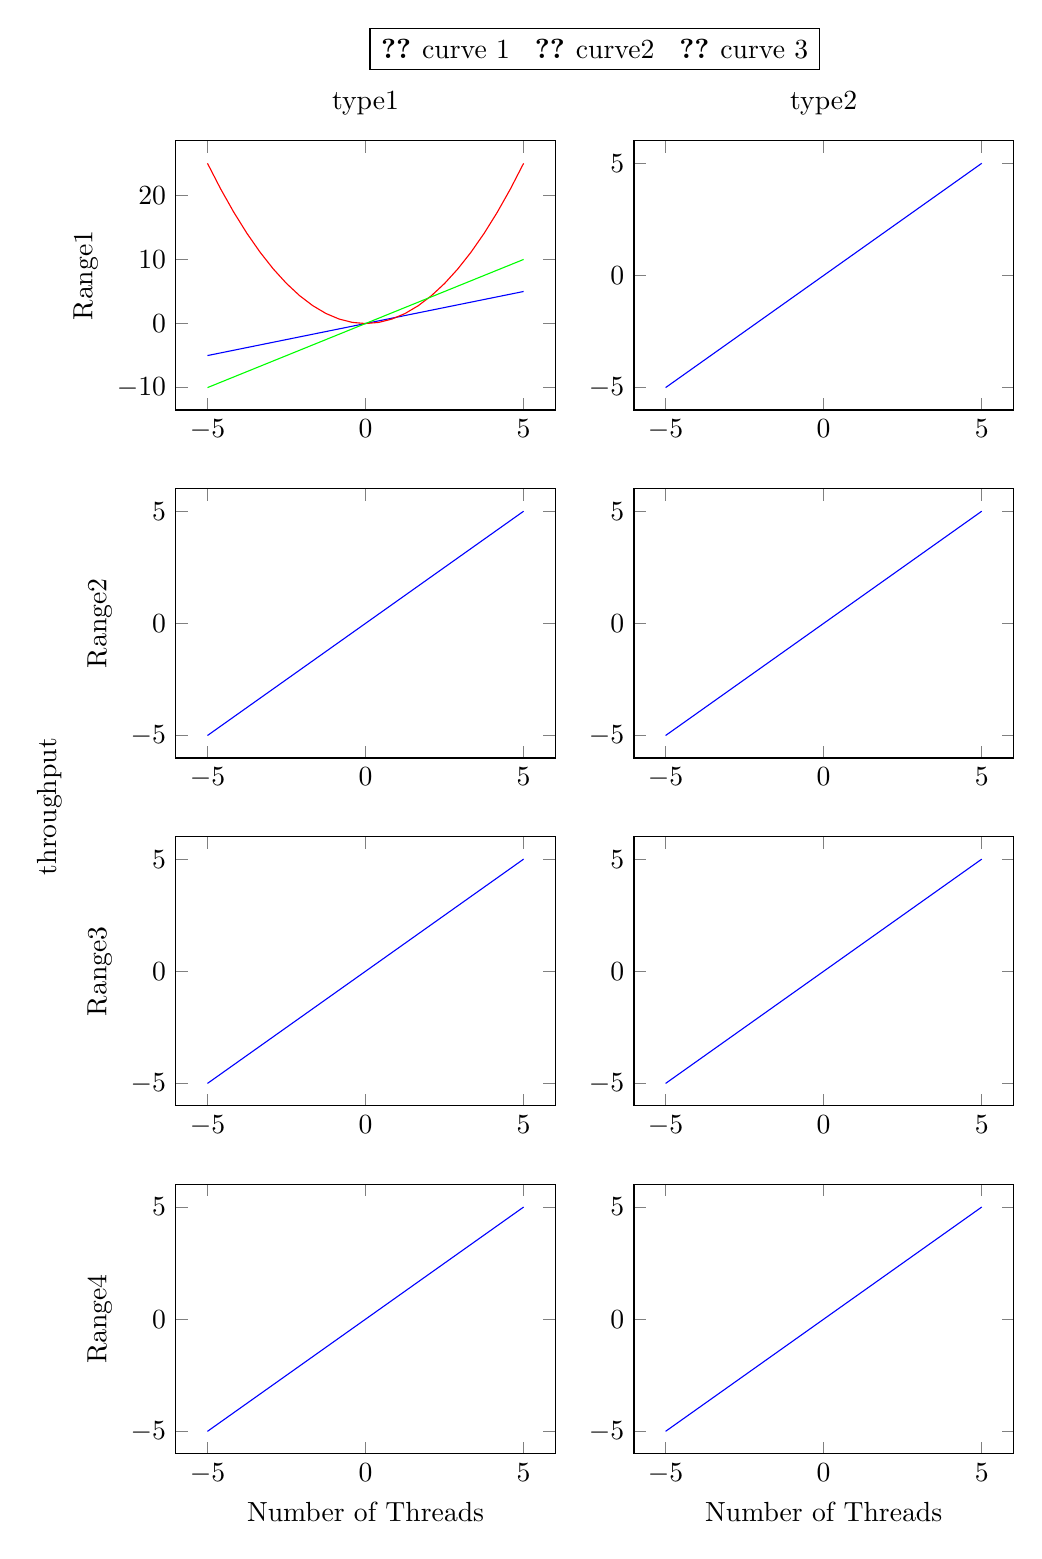
\begin{tikzpicture}
    \begin{groupplot}[group style={
                      group name=myplot,
                      group size= 2 by 4},height=5cm,width=6.4cm]
        \nextgroupplot[title=type1,ylabel={Range1 }]
                \addplot[blue] {x};\label{plots:plot1}
                \addplot[red] {x^2};\label{plots:plot2}
                \addplot[green] {2*x};\label{plots:plot3}
        \nextgroupplot[title=type2]
                \addplot[blue]{x};
        \nextgroupplot[ylabel={Range2 }]
                \addplot[blue]{x};
        \nextgroupplot
                \addplot[blue]{x};
        \nextgroupplot[ylabel={Range3 }]
                \addplot[blue]{x};
        \nextgroupplot
                \addplot[blue]{x};
        \nextgroupplot[xlabel={Number of Threads},ylabel={Range4 }]
                \addplot[blue]{x};
        \nextgroupplot[xlabel={Number of Threads}]
                \addplot[blue]{x};
    \end{groupplot}
    \path (myplot c1r1.outer north west)% plot in column 1 row 1
          -- node[anchor=south,rotate=90] {throughput}% label midway
          (myplot c1r4.outer south west)% plot in column 1 row 4
    ;
% legend
\path (myplot c1r1.north west|-current bounding box.north)--
      coordinate(legendpos)
      (myplot c2r1.north east|-current bounding box.north);
\matrix[
    matrix of nodes,
    anchor=south,
    draw,
    inner sep=0.2em,
    draw
  ]at([yshift=1ex]legendpos)
  {
    \ref{plots:plot1}& curve 1&[5pt]
    \ref{plots:plot2}& curve2&[5pt]
    \ref{plots:plot3}& curve 3\\};
\end{tikzpicture}
\end{document} 